
%%%%%%%%%%%%%%%%%%%%%%%%%%%%%%%%%%%%%%%%%
% Beamer Presentation
% LaTeX Template
% Version 1.0 (10/11/12)
%
% This template has been downloaded from:
% http://www.LaTeXTemplates.com
%
% License:
% CC BY-NC-SA 3.0 (http://creativecommons.org/licenses/by-nc-sa/3.0/)
%
%%%%%%%%%%%%%%%%%%%%%%%%%%%%%%%%%%%%%%%%%

%----------------------------------------------------------------------------------------
%	PACKAGES AND THEMES
%----------------------------------------------------------------------------------------

\documentclass{beamer}
\setbeameroption{show notes}
\mode<presentation> {

% The Beamer class comes with a number of default slide themes
% which change the colors and layouts of slides. Below this is a list
% of all the themes, uncomment each in turn to see what they look like.

%\usetheme{default}
%\usetheme{AnnArbor}
%\usetheme{Antibes}
%\usetheme{Bergen}
%\usetheme{Berkeley}
%\usetheme{Berlin}
%\usetheme{Boadilla}
%\usetheme{CambridgeUS}
%\usetheme{Copenhagen}
%\usetheme{Darmstadt}
%\usetheme{Dresden}
%\usetheme{Frankfurt}
%\usetheme{Goettingen}
%\usetheme{Hannover}
%\usetheme{Ilmenau}
%\usetheme{JuanLesPins}
%\usetheme{Luebeck}
\usetheme{Madrid}
%\usetheme{Malmoe}
%\usetheme{Marburg}
%\usetheme{Montpellier}
%\usetheme{PaloAlto}
%\usetheme{Pittsburgh}
%\usetheme{Rochester}
%\usetheme{Singapore}
%\usetheme{Szeged}
%\usetheme{Warsaw}

% As well as themes, the Beamer class has a number of color themes
% for any slide theme. Uncomment each of these in turn to see how it
% changes the colors of your current slide theme.

%\usecolortheme{albatross}
\usecolortheme{beaver}
%\usecolortheme{beetle}
%\usecolortheme{crane}
%\usecolortheme{dolphin}
%\usecolortheme{dove}
%\usecolortheme{fly}
%\usecolortheme{lily}
%\usecolortheme{orchid}
%\usecolortheme{rose}
%\usecolortheme{seagull}
%\usecolortheme{seahorse}
%\usecolortheme{whale}
%\usecolortheme{wolverine}

%\setbeamertemplate{footline} % To remove the footer line in all slides uncomment this line
%\setbeamertemplate{footline}[page number] % To replace the footer line in all slides with a simple slide count uncomment this line

%\setbeamertemplate{navigation symbols}{} % To remove the navigation symbols from the bottom of all slides uncomment this line
}

\usepackage{graphicx} % Allows including images
\usepackage{booktabs} % Allows the use of \toprule, \midrule and \bottomrule in tables
\usepackage{listings, color}
\usepackage{lstautogobble}

\definecolor{forestgreen}{RGB}{34,139,34}
\definecolor{orangered}{RGB}{239,134,64}
\definecolor{darkblue}{rgb}{0.0,0.0,0.6}
\definecolor{gray}{rgb}{0.4,0.4,0.4}

\newif\ifcomplete
\completetrue


\lstdefinestyle{java}{language=Java,
                basicstyle=\footnotesize\ttfamily,
                keywordstyle=\footnotesize\color{blue}\ttfamily,
								breaklines=true,
								breakatwhitespace=true,
								tabsize=2,
								columns=fullflexible,
								autogobble=true,
								showstringspaces=false,
}

\lstdefinestyle{XML}
{	basicstyle=\tiny\ttfamily,
  columns=fullflexible,
  showstringspaces=false,
  commentstyle=\color{gray}\upshape
  morestring=[b]",
  morestring=[s]{>}{<},
  morecomment=[s]{<?}{?>},
  stringstyle=\color{black},
  identifierstyle=\color{darkblue},
  keywordstyle=\color{forestgreen},
  morekeywords={xml,xmlns,version,type,android}% list your attributes here
}

\newcommand{\act}{\texttt{Activity}}

\newcommand{\jcode}[1]{\textcolor{darkblue}{\texttt{#1}}}

\graphicspath{ {./images/} }

%----------------------------------------------------------------------------------------
%	TITLE PAGE
%----------------------------------------------------------------------------------------

\title[\LaTeX\ en Beamer]{\LaTeX\ en Beamer} % The short title appears at the bottom of every slide, the full title is only on the title page

\author{Jens Buysse} % Your name
\institute[HoGent] % Your institution as it will appear on the bottom of every slide, may be shorthand to save space
{
Hogeschool Gent \\ % Your institution for the title page
\medskip
\textit{jens.buysse@hogent.be} % Your email address
}
\date{\today} % Date, can be changed to a custom date

\begin{document}

\begin{frame}
\titlepage % Print the title page as the first slide
\end{frame}



%----------------------------------------------------------------------------------------
%	PRESENTATION SLIDES
%----------------------------------------------------------------------------------------

\section{\LaTeX{} wat is dat nu?}

\begin{frame}
	\frametitle{Bij \LaTeX\ denk ik aan \dots}
	
	\begin{figure}
		\centering
			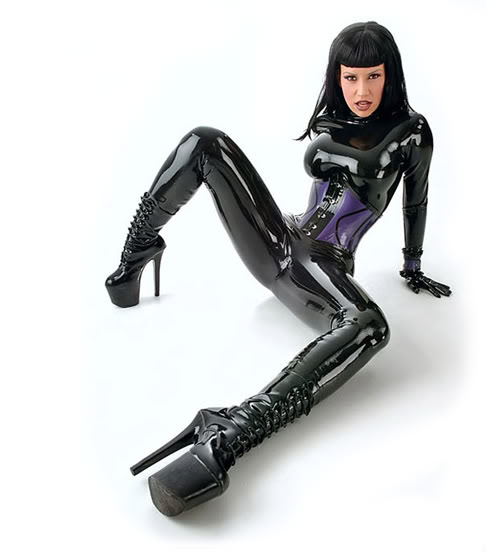
\includegraphics[width=0.65\textwidth]{images/latex.jpg}
		\label{fig:latex}
	\end{figure}
	
\end{frame}

\begin{frame}
\frametitle{Overview} % Table of contents slide, comment this block out to remove it
\tableofcontents % Throughout your presentation, if you choose to use \section{} and \subsection{} commands, these will automatically be printed on this slide as an overview of your presentation
\end{frame}

\begin{frame}
	\frametitle{\LaTeX\ overzicht}
	
	\begin{itemize}
		\item \LaTeX\ is een documentverwerkingssysteem dat toelaat om je op de inhoud te concentreren. Het systeem zelf zorgt voor de layout. 
		\pause
		\item \LaTeX\ is declaratief: aan de hand van instructies en macro's vertel je de compiler wat je wil. Die zal op zijn beurt uw document genereren. 
		\pause
		\item \LaTeX\ is uitermate geschikt voor grote en complexe teksten (thesis, PhD \dots). 
		\pause 
		\item Verder is een onderdeel, BiBTeX, een uitstekende manier om literatuurlijsten bij te houden in je werk.
		\pause
		\item \LaTeX\ is de de facto standaard voor wetenschappelijk schrijven
	\end{itemize}
\end{frame}

\begin{frame}
	\frametitle{Enkele voordelen van \LaTeX}
	
	\begin{itemize}
		\item Automatische generatie van TOC
		\item Refereren wordt correct voor je gedaan
		\item Secties en subsecties worden correct voor je beheerd
		\item Makkelijk om (pseudo)code en wiskunde te noteren
		\item Conditionele compilatie
		\item Je kan eigen macro's schrijven en het jezelf makkelijk maken
		\item Generatie van professionele documenten (pdf)
		\item Veel extra packages die je kunnen helpen
		\item \dots
	\end{itemize}
\end{frame}

\begin{frame}
	\frametitle{Enkele nadelen van \LaTeX}
		\begin{itemize}
		\item Weinig zeggenschap over layout - wanneer dit de focus is beter ander programma
		\item Een compleet nieuwe layout defini\"eren is tijdrovend en moeilijk
		\item Heel moeilijk om ongestructureerde documenten te maken
		\item Vergt wat moeite in het begin 
		\item Sommige zaken zijn intuitief moeilijk (bv. tabellen maken)
			\end{itemize}
\end{frame}

\begin{frame}
	\frametitle{\LaTeX\ leercurve}
	
	\begin{figure}
		\centering
			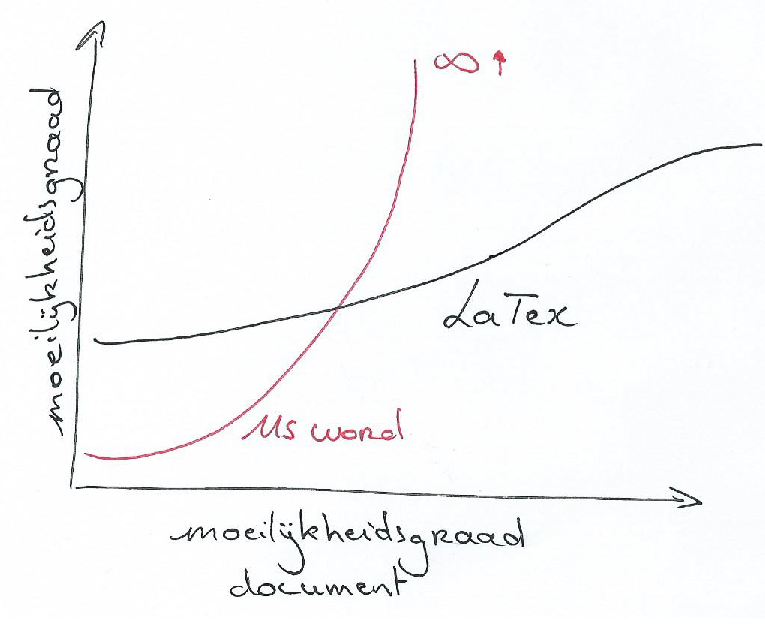
\includegraphics[width=0.75\textwidth]{images/learningCurve.png}
		\label{fig:learningCurve}
	\end{figure}
	
\end{frame}
%
\section{Overtuigd! Maar wat is Beamer dan?}

\begin{frame}
	\frametitle{Overtuigd! Maar wat is Beamer dan?}
	
	\begin{itemize}
		\item Beamer is een packages uit \LaTeX\ waarmee je op dezelfde gestructureerde manier presentaties kan maken.
		\pause
		\item Ken je \LaTeX\ $\Rightarrow$ dan kan je beamer
		\pause
		\item Alle voordelen van \LaTeX\ worden dus overgenomen
	\end{itemize}
\end{frame}

\section{Genoeg gezever! Ik wil er gewoon aan beginnen!!!}

\begin{frame}
	\frametitle{Genoeg gezever! Ik wil er gewoon aan beginnen !!!}
	
	
	\begin{figure}
		\centering
			
\includegraphics[width=0.75\textwidth]{images/letsDoThis.jpg}
		\label{fig:letsDoThis}
	\end{figure}
	
\end{frame}

\end{document} 
